\subsection{Overview}
The behavior of xenon is of principal importance in the prediction and description of nuclear reactor behavior.  This document discusses the relevant features, governing equations, and constitutive formula involved in the analysis of xenon in a Molten Salt Reactor (MSR).  This document is designed to be used in conjunction with the Oak Ridge reports ORNL-4069, ORNL-TM-3464, and the appendix of ORNL-TM-4541. \cite{ORNL4069} \cite{ORNLTM3464} \cite[p. 170]{Robertson1971}

A MSR uses circulating alkali fluoride fuel salt melt as both a fuel matrix and a working fluid. MSR development started in the 1950s at the Oak Ridge National Laboratory (ORNL) in the United States.  This effort reached apogee with the design, development, and subsequent operation of the Molten Salt Reactor Experiment (MSRE) in the 1960s.  The MSR program at ORNL resulted in several conceptual designs of large MSR power systems,  the final one being the Denatured Molten Salt Reactor (DMSR) published in the 1980s.  Details about the history of the MSR program at ORNL are documented by MacPherson and Dolan \cite{MacPherson1985} \cite[p. 2]{Dolan2017} Renewed interest of MSRs is coincident with their inclusion among the Generation IV concepts (GenIV), see Serp. \cite{Serp2014}

For our purposes, let us undergo a brief familiarization with the structural and process components of a simple single-fluid MSR. The description hereafter is not specific to any particular MSR concept. The description stated hereafter is a Technological Level description using the terminology of Lorenz; that is, it is a description of the system at level of components, which are given as \textit{black-boxes}.\cite{Lorenz1996}
The key components of an MSR are shown in Figure \ref{MSRLoop}.
\label{MSRLoop}
\begin{figure}[ht]
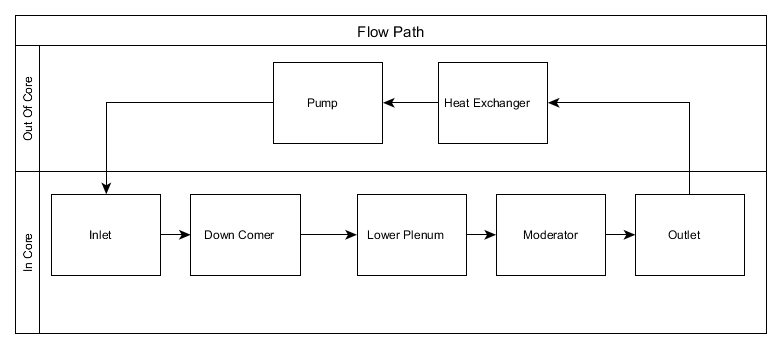
\includegraphics[width=\textwidth,height=\textheight,keepaspectratio]{MSRLoop.png} 
\caption{MSR Flow Path}
\end{figure}

Fuel enters the reactor vessel through the inlet and moves down to the lower plenum via the down comer.  Once in the lower plenum, the fuel salt intramixes and travels up the fuel channels which have been cut into graphite stringers.  The graphite stringers constitute the moderator. When within the moderating region, the fuel undergoes fission and heat is generated. Once the fuel salt has passed through the fuel channels, it leaves the reactor through the outlet and enters the heat exchanger where it deposits its heat content. The fuel salt then leaves the heat exchanger and enters the fuel pump where momentum is imparted into it from the impeller. The fuel salt then leaves the pump and enters the inlet where the cycle is repeated. Pressure is maintained in reactor vessel via the cover gas in the upper plenum.  Cover gas is injected into the upper plenum via the cover gas inlet and removed via the cover gas outlet.  The entire primary circuit can be divided into in-core and out-of-core volumes. The flow paths through these volumes is illustrated below. The primary circuit will likely also contain additional components, which have not been depicted, including a dedicated gas stripper, equipment to sample salt, adjust chemistry, refuel the reactor, etc.

The migratory behavior of xenon in molten salt is qualitatively different than that in solid fuel.  When the fuel is solid the migration of xenon is of secondary importance to the analysis of xenon behavior. In an MSR, the xenon circulates with the fuel salt, and undergoes a number of mass transfer processes in the various regions of the reactor. This includes a possibility to remove xenon (and other fission gases) off the fuel, which is a unique capability of molten fuel.   After its production via nuclear fission or the decay of iodine, the xenon moves about the reactor dissolved in the salt, in the circulating gaseous voids (bubbles), diffusing into the moderating graphite, or leaving the core to cover gas or through offgasing equipment.  The source, sink and migration processes in MSR xenon theory are summarized in Table \ref{termTable}.
\begin{table}[ht]
\begin{tabularx}{\linewidth}{ |X|X|X| }
  \hline
 \textbf{Source Terms} & \textbf{Sink Terms} & \textbf{Migration Terms} \\
  \hline 
  Fission Production  & Radioactive Decay  & Mass Transfer to Circulating Voids   \\
  \hline
  Production From Progenitors & Burn Out & Removal via Cover Gas Outlet Line \\
   \hline
    & Removal via Cover Gas Outlet Line & Mass Transfer to Cover Gas \\
   \hline
\end{tabularx}
\caption{Terms in MSR Xenon Analysis }
\label{termTable}
\end{table}






Figure \ref{XeBlocks} shows a qualitative description of processes in MSR xenon theory. $^{135}Xe$  originates from either fission or the $^{135}Xe$  progenitors, $^{135}I$  and $^{135}Te$ . The aforementioned isotopes, henceforth described as \textit{poison species},  are all fission products and are produced in nuclear fission. $^{135}Te$ transmutes into  $^{135}I$ which transmutes into  $^{135}Xe$.$^{135}Xe$  transmutes into $^{135}Cs$. All the previously mentioned decay processes are facilitated through beta minus decay.  The poison species are all formed inside of the fuel salt.  The  $^{135}Te$ and  $^{135}I$ remain in solution in the fuel salt, whereas the  $^{135}Xe$ is able to migrate from the fuel salt to the cover-gas, circulating voids (bubbles), and cover-gas due to its noble and gaseous nature. There may also be mass transfer directly from bubbles to the graphite.  The absorption cross sections of  $^{135}Te$ and  $^{135}I$ are assumed to be negligible.  In addition to burn-up and radioactive decay,  $^{135}Xe$ may be removed from the system from removal of the cover-gas.  There is a distinction in terminology between diffusive off-gassing and mechanical sparging.  In off-gassing, diffusion drives dissolved gas past an interface whereas sparging refers to a mechanical gas removal process. An example of sparging is the xenon spray-ring in the Molten Salt Reactor Experiment (described later).  The ORNL literature uses the term stripping occasionally in place of sparging.

\begin{figure}[ht]
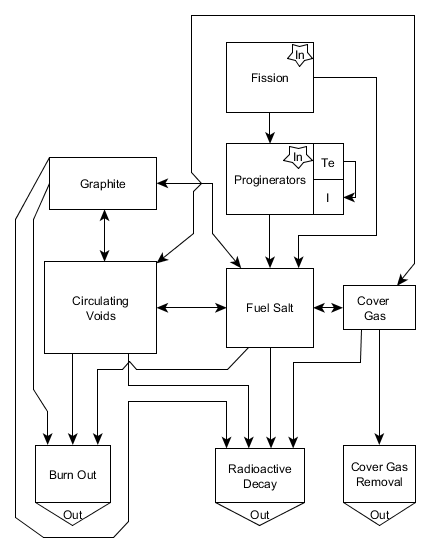
\includegraphics[width=\textwidth,height=\textheight,keepaspectratio]{XeBlocks.png} 
\caption{Xenon Mass Transfer Pathways}
\label{XeBlocks}
\end{figure}